\section{Results}\label{sec:results}

In this Section, we report posterior constraints on the parameters listed in Table~\ref{tab:emulatorparams}.
Section~\ref{sec:cosmo} discusses the results for those parameters which are most strongly constrained by the flux power spectrum data.
These are: the optical depth parameters, $\tau_0$ and $d\tau_0$, the power spectrum parameters, $n_P$ and $A_p$, and the growth function $\Omega_M h^2$.
Section~\ref{sec:astro} then discusses the constraints on the other parameters, and shows the best fit to the mean IGM temperature data.
These are the three parameters defining the He~{\sc{ii}} reionization model, z$^{\text{He~{\sc ii}}}_i$, z$^{\text{He~{\sc ii}}}_f$, and $\alpha_q$; the parameter for the midpoint of H~{\sc{i}} reionization, z$^{\text{H~{\sc i}}}$, the strong absorber models, $\alpha_{LLS}$ and $\alpha_{DLA}$), the Silicon III correction (fSiIII) and the velocity to distance scale parameter $v_{scale}$.
The same chains are used in all sections: we split parameters into two sections merely for readability.
We show the full corner plot, containing all constrained parameters, in Appendix~\ref{sec:full_posteriors}.
Table~\ref{table:parameters} shows marginalised posterior parameter constraints, including the derived parameters $A_s$ and $\sigma_8$. 

% --------------------------------------------------------------------------------------------------

\subsection{Cosmological Parameters}\label{sec:cosmo}

\begin{figure}
    \centering
    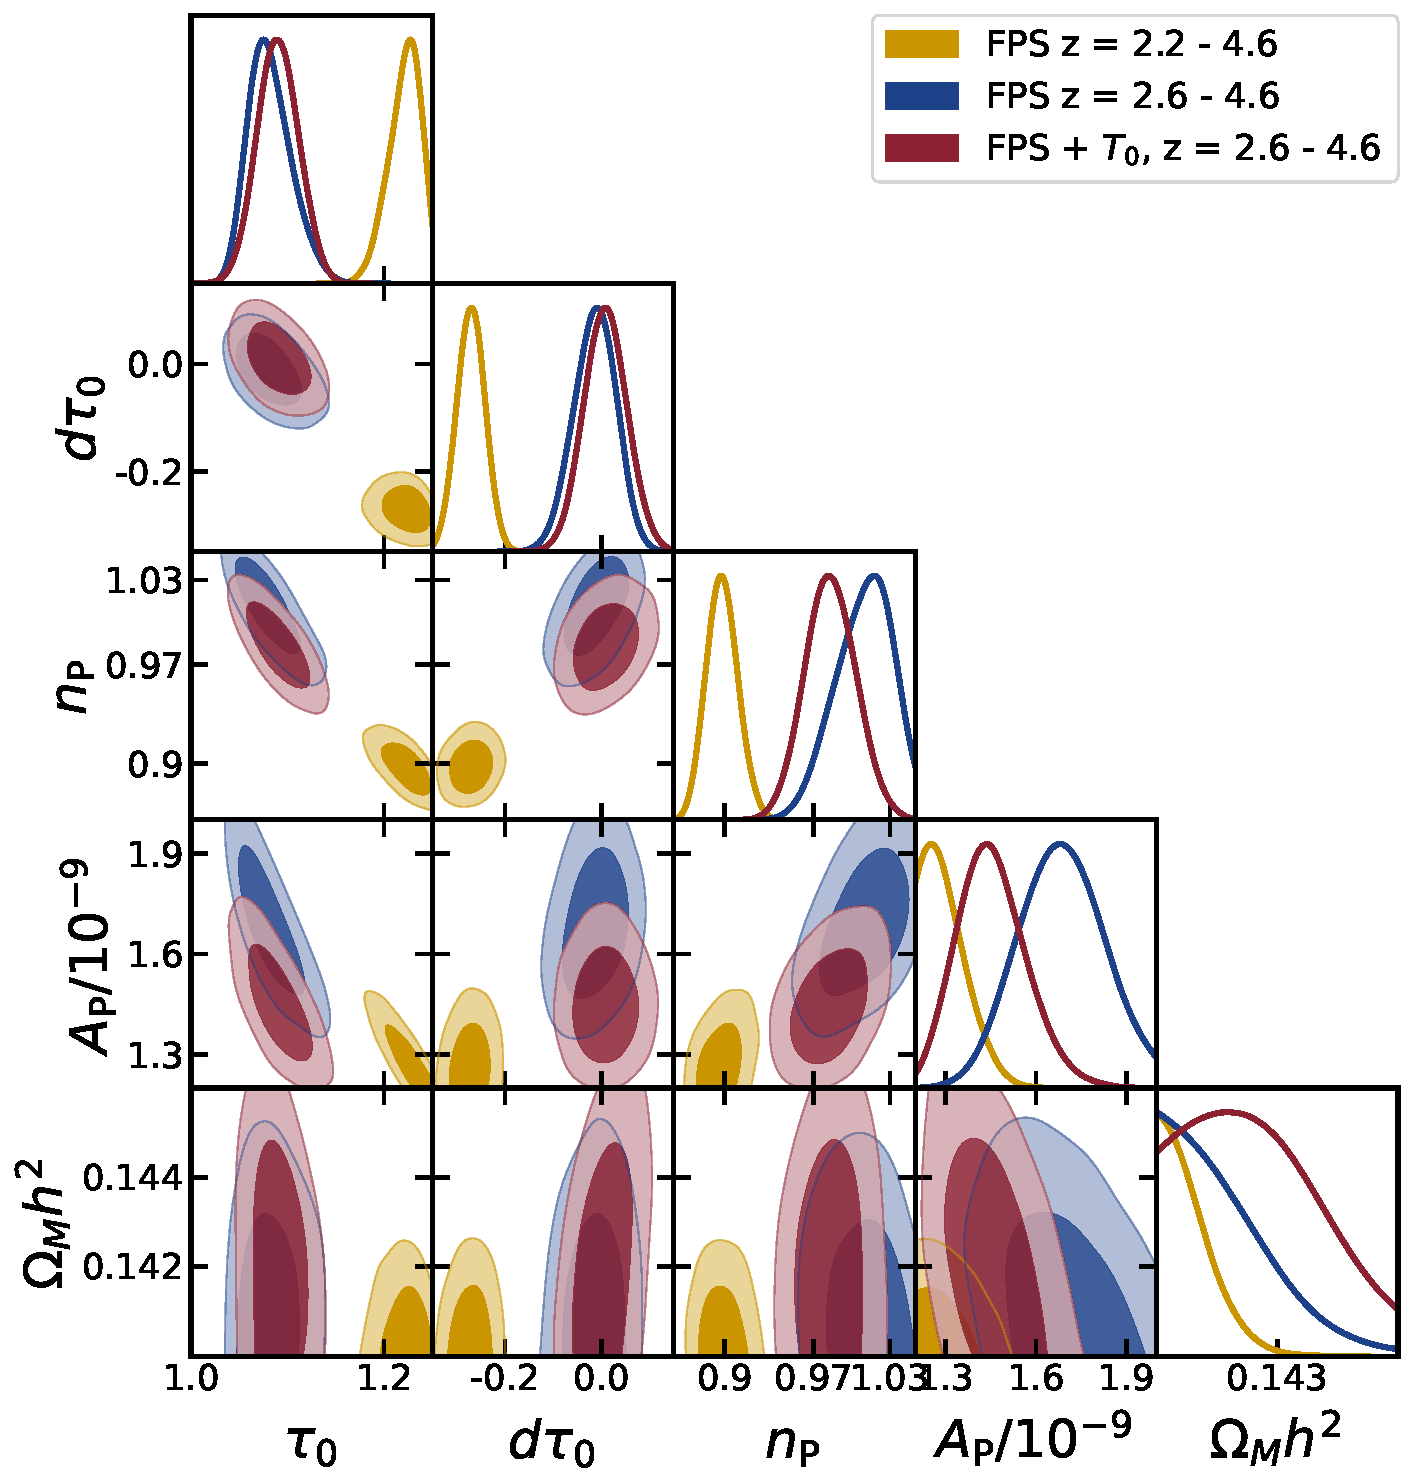
\includegraphics[width=0.75\textwidth]{figures/cosmo_corner.pdf}
    \caption{\label{fig:cosmo_corner}
    Posteriors for the optical depth and power spectrum parameters, $\tau_0$, $d\tau_0$, $n_P$, $A_p$, and $\Omega_M h^2$.
    Results are from three MCMC chains: those labelled `FPS' use the flux power spectrum only.
    These include a chain using the full eBOSS dataset, `FPS $z=2.2-4.6$' (black) and a chain using a limited range eBOSS dataset, found to remove the internal tension (Section~\ref{sec:tension}), `FPS $z=2.6-4.6$' (red).
    The third chain, `FPS $z=2.6-4.6$' (gold), uses the limited range eBOSS dataset but adds the mean IGM temperature constraints.
    Our preferred \maf{what does robust mean here? lowest chi-squared?} \spb{robust is not right, I think I just mean 'preferred', for caption readers who don't read the paper} cosmological constraints are the red chain, `FPS $z=2.6-4.6$'.
    }
\end{figure}

%\begin{table}
%\centering
%\def\arraystretch{1.2}
%\begin{tabular} {| l | c | c |}
%\hline
% Parameter &  68\% limits &  95\% limits\\
%\hline
%$d\tau_0        $ & $-0.240\pm 0.030           $    & $-0.240^{+0.058}_{-0.059}  $   \\
%$\tau_0         $ & $1.214^{+0.013}_{-0.010}   $    & $1.214^{+0.022}_{-0.024}   $   \\
%$n_\mathrm{P}   $ & $0.891\pm 0.011            $    & $0.891^{+0.021}_{-0.020}   $   \\
%$A_\mathrm{P}/10^{-9}$ & $< 1.28 $    & $< 1.36$   \\
%$z^{HeII}_i     $ & $> 4.07                    $    & $> 4.02                    $   \\
%$z^{HeII}_f     $ & $< 2.68                    $    & $< 2.80                    $   \\
%$\alpha_{q}     $ & $> 2.41                    $    & $> 2.28                    $   \\
%$v_\mathrm{scale}$ & $0.6943^{+0.0070}_{-0.0086}$   & $0.694^{+0.018}_{-0.016}  $   \\
%$\Omega_M h^2   $ & $0.14143^{+0.00063}_{-0.00097}$ & $< 0.143                   $   \\
%$z^{HI}         $ & $> 7.79                    $    & $> 7.54                    $   \\
%$\alpha_{lls}   $ & $0.039^{+0.017}_{-0.019}   $    & $0.039^{+0.037}_{-0.034}   $   \\
%$\alpha_{dla}   $ & $-0.0073\pm 0.0032         $    & $-0.0073^{+0.0062}_{-0.0064}$  \\
%$f_\mathrm{SiIII}         $ & $0.00881\pm 0.00040        $    & $0.00881^{+0.00076}_{-0.00077}$\\
%\hline
%$A_\mathrm{s}/10^{-9}      $ & $1.709^{+0.063}_{-0.089}$ & $1.71^{+0.16}_{-0.15}$\\
%$\sigma_8                  $ & $0.713^{+0.012}_{-0.018}$  & $0.713^{+0.032}_{-0.028}$\\
%\hline
%\end{tabular}
%\caption{\label{table:z22z46parameters}
%Constraints from the flux power spectrum using the full redshift range, $z = 2.2 - 4.6$. Maximum posterior values, $68\%$ and $95\%$ confidence limits are shown. $A_s$ and $\sigma_8$ are derived.
%}
%\end{table}

%\begin{table}
%	\centering
%      \def\arraystretch{1.2}
%\begin{tabular} {| l | c | c | c | c|}
%\hline
% Parameter &  FPS  (68\%) &  FPS  (95\%) &  FPS + $T_0$ (68\%) &  FPS + $T_0$  (95\%) \\
%\hline
%$d\tau_0        $ & $-0.006\pm 0.037           $ & $-0.006^{+0.071}_{-0.076}  $  & $0.028\pm 0.036            $ & %$0.028^{+0.070}_{-0.071}   $\\
%$\tau_0         $ & $1.098^{+0.016}_{-0.020}   $ & $1.098^{+0.036}_{-0.033}   $  & $1.093\pm 0.017            $ & %$1.093^{+0.034}_{-0.033}   $\\
%$n_\mathrm{P}   $ & $> 0.969                   $ & $> 0.949                   $  & $0.972^{+0.018}_{-0.0095}  $ & $> 0.948                   $\\
%$A_\mathrm{P}/10^{-9}$ & $1.56\pm 0.12         $ & $1.56^{+0.25}_{-0.23}$        & $1.385^{+0.083}_{-0.11}$   & $< 1.56       $               \\
%$z^{HeII}_i     $ & $> 4.04                    $ & $> 3.95                    $  & $4.037^{+0.052}_{-0.024}   $ & $> 3.97                    $\\
%$z^{HeII}_f     $ & $< 2.76                    $ & $< 2.98                    $  & $2.718\pm 0.044            $ & $2.718^{+0.087}_{-0.087}   $\\
%$\alpha_{q}     $ & $> 2.32                    $ & $> 2.03                    $  & $1.404^{+0.038}_{-0.092}   $ & $< 1.52                    $\\
%$v_\mathrm{scale}$ & $0.691^{+0.011}_{-0.0091}  $ & $0.691^{+0.021}_{-0.022}$    & $0.684^{+0.016}_{-0.0096} $  & $0.684^{+0.021}_{-0.026}   $\\
%$\Omega_M h^2   $ & $0.1425^{+0.0011}_{-0.0015}$ & $0.1425^{+0.0024}_{-0.0024}$ & $0.1427^{+0.0013}_{-0.0018}$ & ---                         \\
%$z^{HI}         $ & $> 7.61                    $ & $> 7.24                    $ & $7.58^{+0.37}_{-0.16}      $ & $> 7.09                    $\\
%$\alpha_{lls}   $ & $0.162\pm 0.029            $ & $0.162^{+0.056}_{-0.057}   $ & $0.191\pm 0.028            $ & $0.191^{+0.054}_{-0.056}   $\\
%$\alpha_{dla}   $ & $-0.0038\pm 0.0060         $ & $-0.0038^{+0.012}_{-0.012}  $ & $-0.0135\pm 0.0054         $ & $-0.014^{+0.010}_{-0.011}  $\\
%$fSiIII         $ & $0.00966\pm 0.00051        $ & $0.00966^{+0.0010}_{-0.0010}$ & $0.00962\pm 0.00051        $ & $0.00962^{+0.0010}_{-0.00099} $ \\
%\hline
%$A_\mathrm{s}/10^{-9}      $ & $1.67^{+0.12}_{-0.13}$ & $1.67^{+0.27}_{-0.24}$ & $1.495^{+0.094}_{-0.12}$ & $1.495^{+0.21}_{-0.20}$\\
%$\sigma_8$ & $0.733\pm 0.026            $ & $0.733^{+0.052}_{-0.049}$ &  $0.696^{+0.021}_{-0.025}   $ & $0.696^{+0.045}_{-0.043}$ \\
%\hline
%\end{tabular}
%\caption{\label{table:parameters}
%Constraints from the flux power spectrum (FPS) and flux power spectrum and mean IGM temperature (FPS + $T_0$) using the reduced redshift range, $z = 2.6 - 4.6$. Maximum posterior values, $68\%$ and $95\%$ confidence limits are shown. $A_s$ and $\sigma_8$ are derived.
%    }
%\end{table}

% \begin{table}
% 	\centering
%       \def\arraystretch{1.6}
% \begin{tabular} {| l | c | c | c|}
% \hline
% Parameter &  FPS $z>2.6$ 68\% (95\%) &  FPS + $T_0$ 68\%, (95\%) & FPS $z>2.2$ 68\%, (95\%) \\
% \hline
% $d\tau_0        $ & $-0.006\pm 0.037$  $\left(^{+0.071}_{-0.076}\right)$                   & $0.028\pm 0.036$            $\left(^{+0.070}_{-0.071}\right)$                   & $-0.240\pm 0.030$     $\left(^{+0.058}_{-0.059}  \right)$   \\
% $\tau_0         $ & $1.098^{+0.016}_{-0.020}$  $\left( ^{+0.036}_{-0.033}\right)$            & $1.093\pm 0.017$       $\left(^{+0.034}_{-0.033}\right)$                   & $1.214^{+0.013}_{-0.010}$   $\left(^{+0.022}_{-0.024}\right)$   \\
% $n_\mathrm{P}   $ & $> 0.969                   $  ($> 0.949                   $)  & $0.972^{+0.018}_{-0.0095}$  ($> 0.948   $)    & $0.891\pm 0.011$            $\left(^{+0.021}_{-0.020}\right)$   \\
% $A_\mathrm{P}/10^{-9}$ & $1.56\pm 0.12$        $\left(^{+0.25}_{-0.23}\right)$        & $1.385^{+0.083}_{-0.11}$   ($< 1.56 $)                   &           $< 1.28 $  ($< 1.36$)   \\
% $\Omega_M h^2   $ & $0.1425^{+0.0011}_{-0.0015}$ $(^{+0.0024}_{-0.0024})$       & $0.1427^{+0.0013}_{-0.0018}$  (---)                              & $0.14143^{+0.00063}_{-0.00097}$ ($< 0.143$)   \\
% $z^{HeII}_i     $ & $> 4.04                    $ $> 3.95                    $  & $4.037^{+0.052}_{-0.024}   $ $(> 3.97 ) $    & $> 4.07                    $  $(> 4.02)$   \\
% $z^{HeII}_f     $ & $< 2.76                    $  $(< 2.98)$                   & $2.718\pm 0.044            $  $\left(^{+0.087}_{-0.087}\right)$    & $< 2.68                    $    $(< 2.80 )$   \\
% $\alpha_{q}     $ & $> 2.32                    $  $(> 2.03)$                   & $1.404^{+0.038}_{-0.092}   $  $(< 1.52 )$              & $> 2.41                    $    $(> 2.28 )                   $   \\
% $z^{HI}         $ & $> 7.61                    $ ($> 7.24 $) & $7.58^{+0.37}_{-0.16}      $ ($> 7.09 $)     & $> 7.79                    $    $(> 7.54 )$   \\
% $v_\mathrm{scale}$ & $0.691^{+0.011}_{-0.0091}  $  $\left(^{+0.021}_{-0.022}\right)$    & $0.684^{+0.016}_{-0.0096} $  $\left(^{+0.021}_{-0.026}\right)$    & $0.6943^{+0.0070}_{-0.0086}$  $\left(^{+0.018}_{-0.016} \right)$     \\
% $\alpha_{lls}   $ & $0.162\pm 0.029   $ $\left(^{+0.056}_{-0.057}\right)$          & $0.191\pm 0.028            $  $\left(^{+0.054}_{-0.056}\right)   $     & $0.039^{+0.017}_{-0.019}   $  $\left(^{+0.037}_{-0.034}\right)$   \\
% $\alpha_{dla}   $ & $-0.0038\pm 0.0060         $ $\left(^{+0.012}_{-0.012}\right)$ & $-0.0135\pm 0.0054         $ $\left(^{+0.010}_{-0.011}\right)  $    & $-0.0073\pm 0.0032         $   $\left(^{+0.0062}_{-0.0064}\right)$  \\
% $f_{SiIII}/10^{-3} $ & $9.66\pm 0.51              $ $\left(^{+1.0}_{-1.0}\right)$              & $9.62\pm 0.51        $       $\left(^{+1.0}_{-0.99}\right) $          & $8.81\pm 0.40        $  $\left(^{+0.76}_{-0.77}\right)$\\
% \hline
% $A_\mathrm{s}/10^{-9}      $ & $1.67^{+0.12}_{-0.13}$ $\left(^{+0.27}_{-0.24}\right)$ & $1.495^{+0.094}_{-0.12}$ $\left(^{+0.21}_{-0.20}\right)$  & $1.709^{+0.063}_{-0.089}$ $\left(^{+0.16}_{-0.15}\right)$   \\
% $\sigma_8$ & $0.733\pm 0.026            $ $\left(^{+0.052}_{-0.049}\right)$ &  $0.696^{+0.021}_{-0.025}   $ $\left(^{+0.045}_{-0.043}\right)$ & $0.713^{+0.012}_{-0.018}$  $\left(^{+0.032}_{-0.028}\right)$  \\
% \hline
% \end{tabular}
% \caption{\label{table:parameters}
% Posterior parameter constraints, including the derived parameters $A_s$ and $\sigma_8$. Maximum posterior values, and $68\%$ confidence limits are shown, with 95\% confidence intervals in brackets. Each column shows a separate chain, from left to right: fits to the flux power spectrum alone from the reduced redshift range $z=2.6 - 4.6$, fits to the flux power spectrum from the reduced redshift range $z=2.6 - 4.6$ and to the mean IGM temperature, and fits to the flux power spectrum alone from the full redshift range $z=2.2 - 4.6$. Single sided limits are shown when one bound is larger than the prior volume of the emulator.
% }
% \end{table}

\begin{table}
	\centering
      \def\arraystretch{1.6}
\begin{tabular} {| l | c | c | c|}
\hline
 & FPS $z>2.6$ & FPS + $T_0$ & FPS $z>2.2$ \\
Parameter & 68\% (95\%) & 68\%, (95\%) & 68\%, (95\%)
\\
\hline
$d\tau_0        $ & $-0.006\pm 0.037$  $\left(^{+0.071}_{-0.076}\right)$                   & $0.028\pm 0.036$            $\left(^{+0.070}_{-0.071}\right)$                   & $-0.240\pm 0.030$     $\left(^{+0.058}_{-0.059}  \right)$   \\
$\tau_0         $ & $1.098^{+0.016}_{-0.020}$  $\left( ^{+0.036}_{-0.033}\right)$            & $1.093\pm 0.017$       $\left(^{+0.034}_{-0.033}\right)$                   & $1.214^{+0.013}_{-0.010}$   $\left(^{+0.022}_{-0.024}\right)$   \\
$n_\mathrm{P}   $ & $> 0.969                   $  ($> 0.949                   $)  & $0.972^{+0.018}_{-0.0095}$  ($> 0.948   $)    & $0.891\pm 0.011$            $\left(^{+0.021}_{-0.020}\right)$   \\
$A_\mathrm{P}/10^{-9}$ & $1.56\pm 0.12$        $\left(^{+0.25}_{-0.23}\right)$        & $1.38^{+0.08}_{-0.11}$   ($< 1.56 $)                   &           $< 1.28 $  ($< 1.36$)   \\
$\Omega_M h^2   $ & $0.1425^{+0.0011}_{-0.0015}$ $(^{+0.0024}_{-0.0024})$       & $0.1427^{+0.0013}_{-0.0018}$  (---)                              & $0.1414^{+0.0006}_{-0.0010}$ ($< 0.143$)   \\
$z^{HeII}_i     $ & $> 4.04                    $ $(> 3.95)                    $  & $4.04^{+0.05}_{-0.02}   $ $(> 3.97 ) $    & $> 4.07                    $  $(> 4.02)$   \\
$z^{HeII}_f     $ & $< 2.76                    $  $(< 2.98)$                   & $2.72\pm 0.04            $  $\left(^{+0.09}_{-0.09}\right)$    & $< 2.68                    $    $(< 2.80 )$   \\
$\alpha_{q}     $ & $> 2.32                    $  $(> 2.03)$                   & $1.40^{+0.04}_{-0.09}   $  $(< 1.52 )$              & $> 2.41                    $    $(> 2.28 )                   $   \\
$z^{HI}         $ & $> 7.61                    $ ($> 7.24 $) & $7.58^{+0.37}_{-0.16}      $ ($> 7.09 $)     & $> 7.79                    $    $(> 7.54 )$   \\
$v_\mathrm{scale}$ & $0.691^{+0.011}_{-0.009}  $  $\left(^{+0.021}_{-0.022}\right)$    & $0.684^{+0.016}_{-0.010} $  $\left(^{+0.021}_{-0.026}\right)$    & $0.694^{+0.007}_{-0.009}$  $\left(^{+0.018}_{-0.016} \right)$     \\
$\alpha_{lls}   $ & $0.162\pm 0.029   $ $\left(^{+0.056}_{-0.057}\right)$          & $0.191\pm 0.028            $  $\left(^{+0.054}_{-0.056}\right)   $     & $0.039^{+0.017}_{-0.019}   $  $\left(^{+0.037}_{-0.034}\right)$   \\
$\alpha_{dla}/10^{-2}   $ & $-0.4\pm 0.6         $ $\left(^{+1.2}_{-1.2}\right)$ & $-1.3\pm 0.5         $ $\left(^{+1.0}_{-1.1}\right)  $    & $-0.7\pm 0.3         $   $\left(^{+0.6}_{-0.6}\right)$  \\
$f_{SiIII}/10^{-3} $ & $9.66\pm 0.51              $ $\left(^{+1.0}_{-1.0}\right)$              & $9.62\pm 0.51        $       $\left(^{+1.0}_{-0.99}\right) $          & $8.81\pm 0.40        $  $\left(^{+0.76}_{-0.77}\right)$\\
\hline
$A_\mathrm{s}/10^{-9}      $ & $1.67^{+0.12}_{-0.13}$ $\left(^{+0.27}_{-0.24}\right)$ & $1.49^{+0.09}_{-0.12}$ $\left(^{+0.21}_{-0.20}\right)$  & $1.71^{+0.06}_{-0.09}$ $\left(^{+0.16}_{-0.15}\right)$   \\
$\sigma_8$ & $0.733\pm 0.026            $ $\left(^{+0.052}_{-0.049}\right)$ &  $0.696^{+0.021}_{-0.025}   $ $\left(^{+0.045}_{-0.043}\right)$ & $0.713^{+0.012}_{-0.018}$  $\left(^{+0.032}_{-0.028}\right)$  \\
\hline
\end{tabular}
\caption{\label{table:parameters}
\maf{I did some rounding on these values -- original is commented out above} \spb{Thanks!}
Posterior parameter constraints, including the derived parameters $A_s$ and $\sigma_8$.
Maximum posterior values, and $68\%$ confidence limits are shown, with $95\%$ confidence intervals in brackets.
Each column shows a separate chain, from left to right: fits to the flux power spectrum alone from the reduced redshift range $z=2.6 - 4.6$, fits to the flux power spectrum from the reduced redshift range $z=2.6 - 4.6$ and the mean IGM temperature, and fits to the flux power spectrum alone from the full redshift range $z=2.2 - 4.6$.
Single sided limits are shown when one bound is larger than the prior volume of the emulator.
}
\end{table}


\begin{figure}
    \centering
    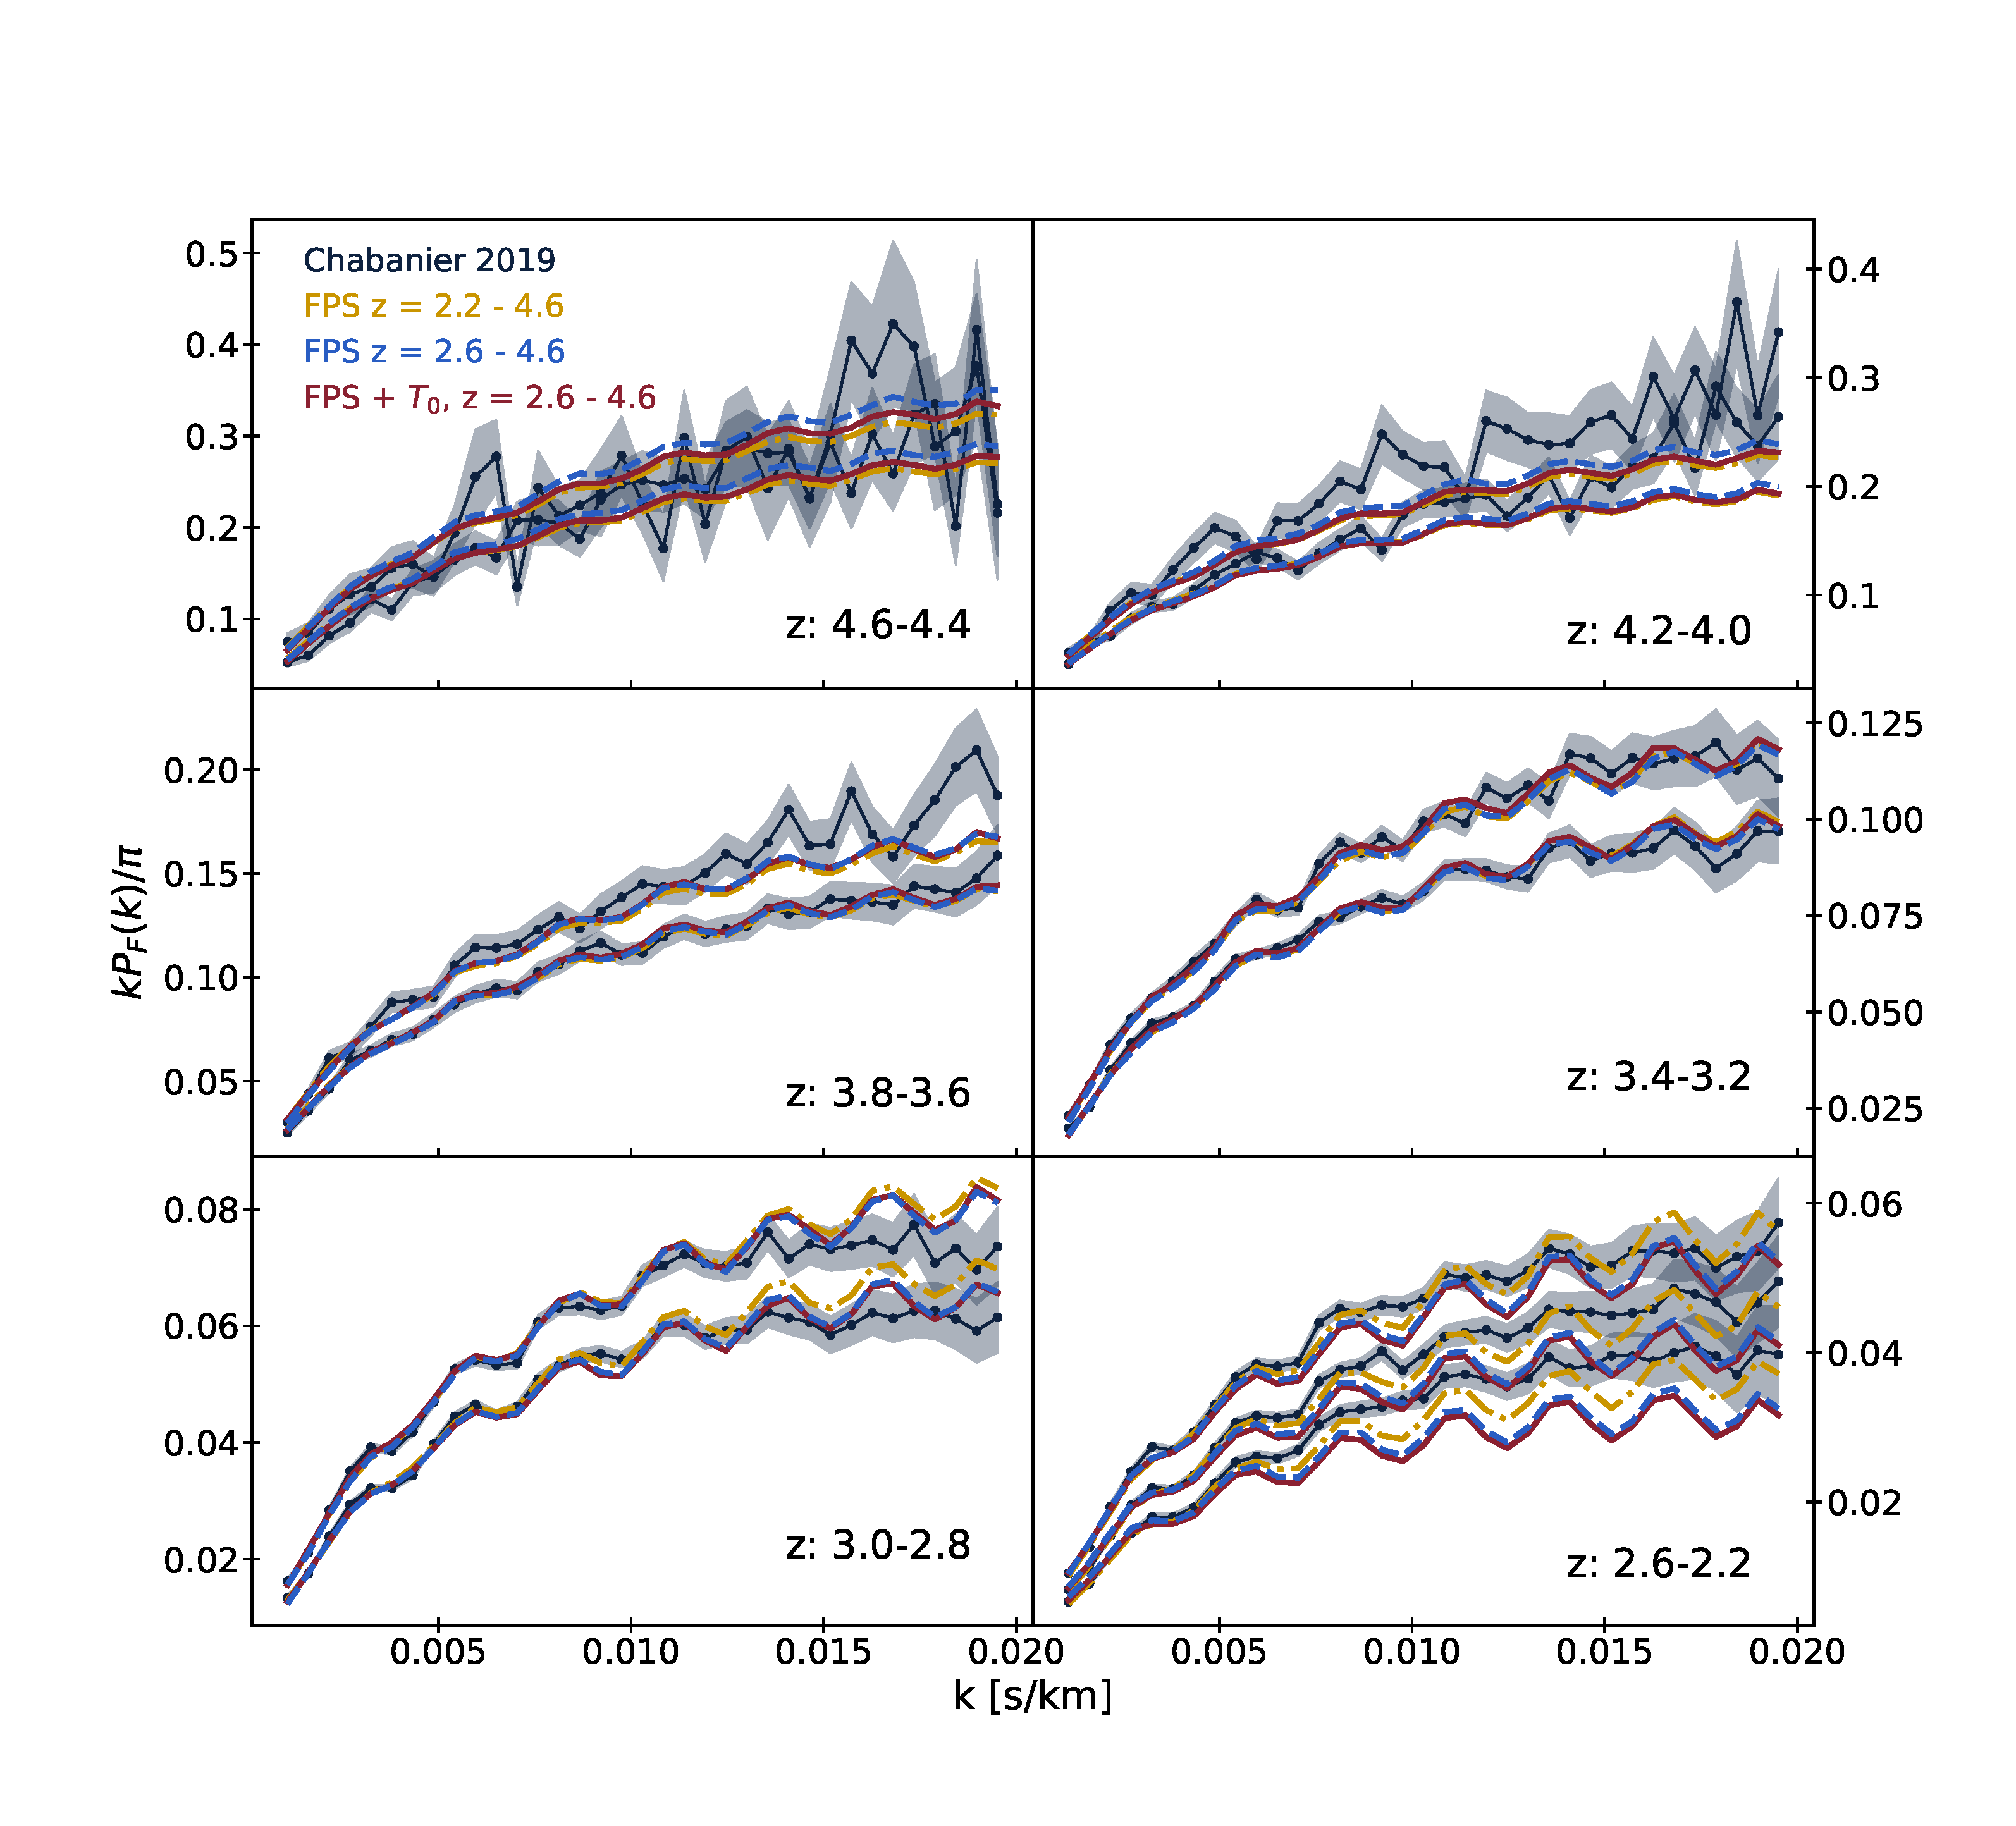
\includegraphics[width=\textwidth]{figures/fps_data_fit.pdf}
    \caption{\label{fig:fps_data}
    \maf{I updated this figure to fix a few visual things, otherwise it is unchanged}\spb{You made it look much nicer!}
    Observed \lya forest flux power spectrum \cite{2019JCAP...07..017C}, from $z=4.6$ to $z=2.2$ (black lines and circles, with shading corresponding to one sigma uncertainty).
    Also shown are three predictions for the \lya forest flux power spectrum from our multi-fidelity emulator corresponding to the maximum posterior input parameters compiled in Table~\ref{table:parameters}.
    The negative of the log-likelihood for these fits is compiled in Table~\ref{table:chi2}.
    }
\end{figure}

Figure~\ref{fig:cosmo_corner} shows the results of our chains for the cosmological parameters.
We show three MCMC chains.
Two chains are fit to the eBOSS flux power spectrum data only.
The first fits to the full redshift range measured by eBOSS, $z=2.2 - 4.6$ (black), while the second fits a limited redshift range $z=2.6 - 4.6$ (red).
The third chain uses the limited redshift range eBOSS dataset but adds the mean IGM temperature likelihood.
The chain including the $z < 2.6$ data prefers lower $n_P$, lower $A_P$ and higher $\tau_0$ than the reduced redshift range.
Figure~\ref{fig:fps_data} shows that the shift in posterior parameters is driven by the fit.
The best-fit flux power spectrum to the data at $z \geq 2.6$ is a poor fit to the flux power spectra measured at $z=2.2$ and $z=2.4$.
Since the lowest redshift bins have the smallest statistical error, when they are included they drive the best-fit flux power spectrum to a region which is a poorer fit to the higher redshift data.
We confirmed that a chain which included the $z=2.4$ bin but not the $z=2.2$ bin produced posterior constraints mid-way between the chain including $z=2.2-4.6$ and the chain including $z=2.6-4.6$.
Table~\ref{table:chi2} shows this quantitatively.
The chains which fit to $z > 2.6$ are a poor fit to the lowest two redshift bins.
The chain fitting to $z=2.2$ is a better fit to these bins, at the cost of an overall worse fit to most higher redshifts.
The total $\chi^2$ per degree of freedom for the reduced redshift chains is close to $1.03$, indicating a good fit, while the full reduced range has a $\chi^2/$dof of $1.15$. 
There is thus an internal tension in the eBOSS dataset, when compared to our model, driven by the lowest two redshift bins.
We discuss possible reasons for this tension in Section~\ref{sec:tension} and compare to the results of earlier analyses further in Section~\ref{sec:comparison}.
It is important not to over-interpret the posterior constraints from the $z=2.2-4.6$ chain.
When there is an internal tension in the data and the overall reduced $\chi^2$ is poor, the posteriors can be driven by noise in the dataset and may not be meaningful.

We also checked for other redshift bins where the fit is poor.
Visually, Figure~\ref{fig:fps_data} suggests that the fit is poor for $z=4.0$ and $z=4.2$.
The reduced $\chi^2$ in Table~\ref{table:chi2} is moderately higher than $1$, but not significantly so, as the statistical errors are also large.
It is possible that some element of the covariance matrix, theoretical or systematic, is moderately underestimated in these bins.
The $z=2.6$ has a slightly elevated $\chi^2$/dof in the reduced redshift range chains, which may suggest that whatever causes the low redshift tension still has a small effect at $z=2.6$.  
%We ran chains which fit to each redshift bin individually, finding that the lowest two redshift bins were still discrepant with the others.

\begin{table}
	\centering
     \def\arraystretch{1.2}
     \begin{tabular}{|c|c|c|c|c|c|c|c|}
		\hline
		Redshift & $4.6$ & $4.4$ & $4.2$ & $4.0$ & $3.8$ & $3.6$ & $3.4$\\
		\hline
        FPS $z: 2.2-4.6$ & $1.08$ & $1.03$ & $1.46$ & $1.79$ & $0.87$ & $0.51$ & $0.63$ \\
        FPS $z: 2.6-4.6$ & $1.22$ & $0.85$ & $1.20$ & $1.40$ & $0.74$ & $0.36$ & $0.69$\\
        FPS $+ T_0$ $z: 2.6-4.6$ & $1.19$ & $0.85$ & $1.28$ & $1.46$ & $0.80$ & $0.31$ & $0.73$ \\
        \hline
        Redshift & $3.2$ & $3.0$ & $2.8$ & $2.6$ & $2.4$ & $2.2$ & Total \\
		\hline
        FPS $z: 2.2-4.6$ & $0.83$ & $1.82$ & $1.64$ & $0.98$ & $0.99$ & $1.36$ & $1.15$ \\
        FPS $z: 2.6-4.6$ & $0.76$ & $1.35$ & $1.29$ & $1.45$ & $2.97$ & $4.17$ & $1.03$ \\
        FPS $+ T_0$ $z: 2.6-4.6$ & $0.82$ & $1.27$ & $1.22$ & $1.67$ & $3.38$ & $4.51$ & $1.06$\\
  \hline
	\end{tabular}
    \caption{\label{table:chi2}
    $\chi^2$ per degree of freedom for the flux power spectrum for each redshift bin.
    Shown is the likelihood at the best fit parameters in each chain.
    We show chains fitting to the flux power spectrum only at $z=2.2-4.6$, fitting to the flux power spectrum only at $z=2.6-4.6$, and fitting to the flux power spectrum and mean IGM temperature at $z=2.6-4.6$.
    The column labelled 'total' is the total $\chi^2$ per degree of freedom for the redshift bins in the fit (i.e., excluding $z=2.2$ and $z=2.4$ for the last two chains).}
\end{table}

Posterior constraints from the reduced redshift range flux power spectrum data show a mean optical depth in good agreement with other measurements.
As a reminder, these parameters measure deviations from the mean flux relation of Ref.~\cite{2007MNRAS.382.1657K}, so a value of $\tau_0=1$ and $d\tau_0=0$ corresponds to agreement with that model.
The best fit mean flux at $z=3$, $\tau_0 = 1.1$, and the redshift variation $d\tau_0$ is consistent with $0$.
This implies a mean optical depth at $z=3$ of $\tau^{\text{eff}}_{\text{H~{\sc i}}}(z=3) = 0.398$, which is extremely close to the best-fit value of $\tau^{\text{eff}}_{\text{H~{\sc i}}}(z=3) = 0.4$ from Ref.~\cite{2013MNRAS.430.2067B}, and consistent within the error bars with $\tau^{\text{eff}}_{\text{H~{\sc i}}}(z=3) = 0.36 \pm 0.1$ from \cite{2007MNRAS.382.1657K}. 

The slope of the spectral index, $n_P$, is $n_P = 0.972^{+0.018}_{-0.009}$ when using $T_0$ and $n_P > 0.969$ when using only the flux power spectrum, where the upper limit of the prior is consistent at $2\sigma$.
This is consistent with the Planck value of $n_s=0.965 \pm 0.004$ \cite{2020A&A...641A...6P}.
The growth factor, $\Omega_M h^2$, is weakly constrained and not strongly affected by including mean temperature data.
Planck found $\Omega_M h^2 = 0.1424\pm0.001$, which is close to the posterior of our chains.
The primordial power spectrum amplitude is $A_p/10^{-9} = 1.56 \pm 0.12$ for the flux power spectrum reduced redshift result.
The inclusion of the mean temperature shrinks the constraints moderately and shifts the posterior value down by about $1.5 \sigma$.
Table~\ref{table:parameters} shows $A_s$, the power spectrum amplitude measured by Planck on large scales, which is related to $A_P$ via:
\begin{equation}
    A_s = \left(0.4/2\pi\right)^{n_P-1} A_P\,.
\end{equation}

We find $A_s = (1.67 \pm 0.12) \times10^{-9}$ for the flux power spectrum alone and $A_s = (1.5 \pm 0.012 )\times10^{-9}$ when including the mean IGM temperature.
Planck \cite{2020A&A...641A...6P} found a value of $A_s = \left(2.101^{+0.031}_{-0.034}\right)\times10^{-9}$. 
We also derived the value of $\sigma_8$ implied by our parameters by using CLASS in post-processing \cite{2011arXiv1104.2932L}. 
For the flux power spectrum alone, we find $\sigma_8 = 0.733 \pm 0.026$, and when the mean IGM temperature is included, $\sigma_8 = 0.696 \pm 0.025$ (see Table\ref{table:parameters}).
The Planck result is $\sigma_8 = 0.811 \pm 0.006$ \cite{2020A&A...641A...6P}.
We thus measure a power spectrum amplitude around $3-\sigma$ lower than Planck.
Interestingly, the dark energy survey year 3 results measure $\sigma_8 = 0.733^{+0.039}_{-0.049}$ \cite{2022PhRvD.105b3520A}, in strikingly good agreement with our results.

Figure~\ref{fig:fps_data} shows the \lya forest flux power spectrum from \cite{2019JCAP...07..017C}, along with their estimated one sigma uncertainty (black).
Also shown are predictions from our multi-fidelity emulator based on the maximum posterior input parameters from MCMC analysis with only the \lya forest flux power emulator in the full and reduced redshift ranges, and MCMC analysis using both the mean temperature and flux power emulators.
The correlation between \lya and Si~{\sc iii} absorption is visible in the form of regular oscillations in the power spectrum (in Section~\ref{sec:likelihood} we describe the correction we make for Si~{\sc iii}).
The best-fit flux power spectrum is not significantly affected by the inclusion of the $T_0$ data in the likelihood, as is expected if the $T_0$ data mainly breaks degeneracies.

% --------------------------------------------------------------------------------------------------
% --------------------------------------------------------------------------------------------------

\subsection{Reionization and Other Parameters}\label{sec:astro}

\begin{figure}
    \centering
    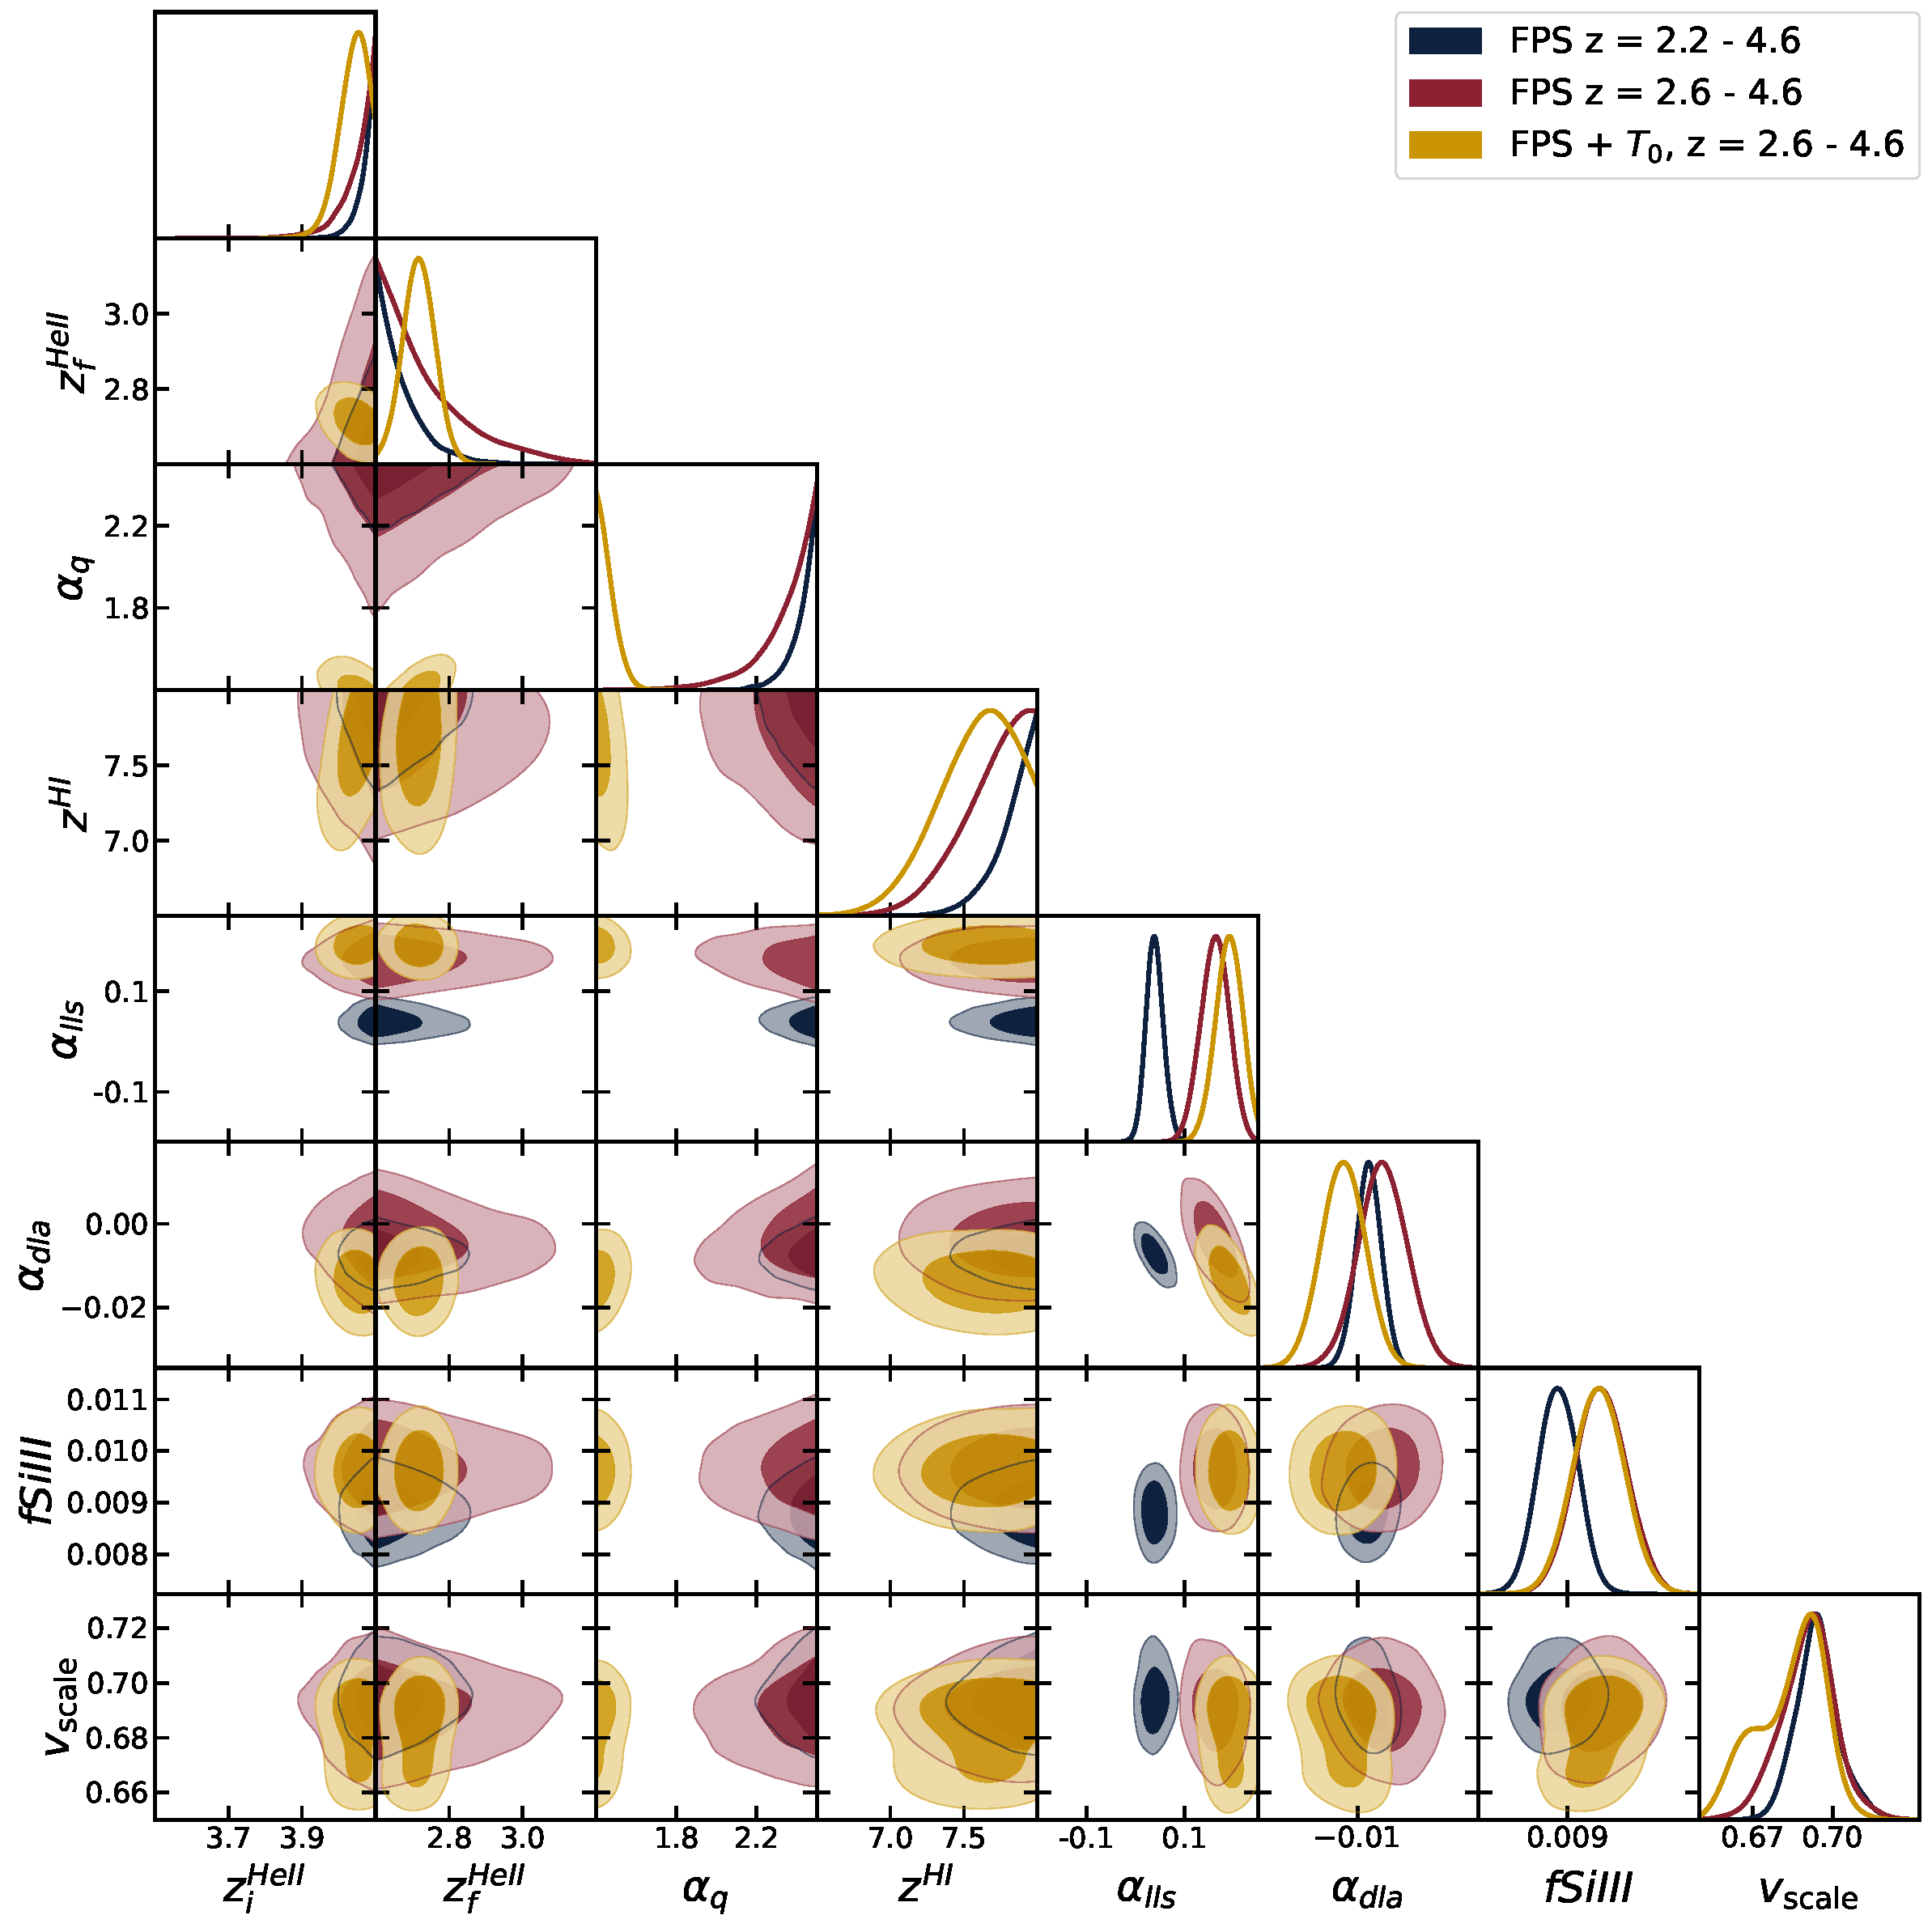
\includegraphics[width=0.85\textwidth]{figures/astro_corner.pdf}
    \caption{\label{fig:astro_corner}
    Posterior constraints for the parameters of the helium reionization model ($z_i^{HeII}$, $z_f^{HeII}$, $\alpha_q$), the hydrogen reionization model ($z^{HI}$), the strong absorber models ($\alpha_{LLS}$, $\alpha_{DLA}$), the Silicon III correction ($f_\mathrm{SiIII}$), and the velocity to distance scale parameter $v_{scale}$.
    Results are from three MCMC chains: those labelled 'FPS' use the flux power spectrum only.
    These are a chain with the full eBOSS dataset, 'FPS $z=2.2 - 4.6$' (black) and a chain with the limited range eBOSS dataset found to remove the internal tension 'FPS $z=2.6 - 4.6$' (red).
    The third chain uses the limited range eBOSS dataset but adds the mean IGM temperature constraints. 'FPS $z=2.6 - 4.6$' (gold).
    }
\end{figure}

\begin{figure}
    \centering
    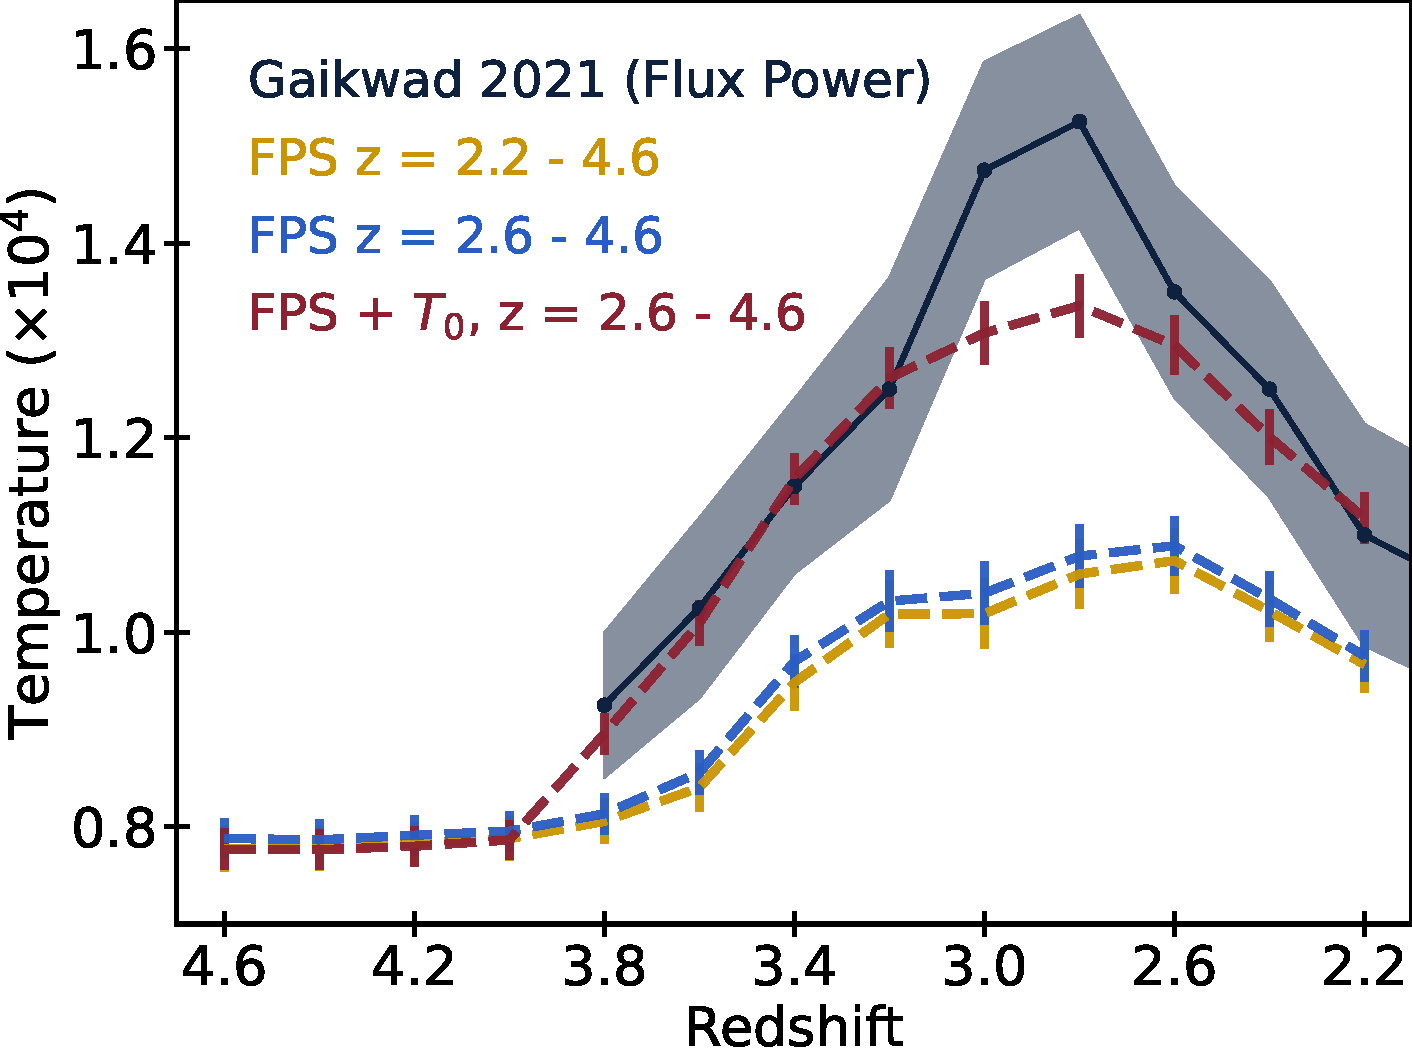
\includegraphics[width=0.75\textwidth]{figures/t0_best_fit.pdf}
    \caption{\label{fig:temp_data}
    \maf{I swapped the colors here for better visibility}
    IGM mean temperatures from \protect\cite{2021MNRAS.506.4389G} (black lines and circles, with shading corresponding to one sigma uncertainty).
    Specifically their temperatures derived from the flux power spectrum calculated using high resolution \lya forest spectra.
    Also shown are predictions for the mean temperature from our multi-fidelity emulator corresponding to the same three maximum posterior input parameters used in Figure~\protect\ref{fig:fps_data}.
    }
\end{figure}

Figure~\ref{fig:astro_corner} shows the other parameters of our model from the same chains as Figure~\ref{fig:cosmo_corner}.
These are: three parameters of the helium reionization model (z$^{\text{He~{\sc ii}}}_i$, z$^{\text{He~{\sc ii}}}_f$, and $\alpha_q$), the midpoint of H~{\sc{i}} reionization z$^{\text{H~{\sc i}}}$, the parameters of the strong absorber model ($\alpha_{LLS}$, $\alpha_{DLA}$), the strength of the metal contamination $f_{SiIII}$ and the box velocity scale $v_{scale}$.

The flux power spectrum data alone prefers an early start to helium reionization, $z_i^{HeII} > 3.9$.
Interestingly, this is in agreement with constraints from the helium \lya forest, where regions of high transmission suggest that HeII reionization has already started at $z = 3.5$ \cite{2016ApJ...825..144W, 2021ApJ...912...38M}.
The mean temperature data reinforce this, but do not substantially shrink constraints, perhaps because the highest redshift mean IGM temperature we fit to is $3.8$, and the flux power spectrum already constrains $z_i^{HeII} > 3.95$ at $95\%$ confidence.
The end of helium reionization, $z_f^{HeII}$, is weakly constrained by the flux power spectrum data alone, but once the mean IGM temperature data is included (importantly, this is the only source of data at $z < 2.6$), constraints tighten to $z=2.7 \pm 0.09$ at $95\%$ confidence.
This is consistent with the He~{\sc{ii}} \lya forest, which suggests an end at $z \leq 2.7$ \cite{2009ApJ...704L..89M, 2011ApJ...733L..24W, 2019ApJ...875..111W}.

The most significant effect of the mean IGM temperature data is on the spectral index during helium reionization, $\alpha_q$.
Smaller values of $\alpha_q$ correspond to a larger heating rate.
The flux power spectrum data prefers a high value of $\alpha_q$, although the constraints are weak.
However, as shown in Figure~\ref{fig:temp_data}, this high value of $\alpha_q$ produces a mean IGM temperature which is extremely low and in clear disagreement with the data from Ref.~\cite{2021MNRAS.506.4389G}.
Figure~\ref{fig:fps_data} shows that the flux power spectrum is not significantly different at the maximum posterior parameters of either chain.
The chains are exploiting a multi-dimensional degeneracy between the helium reionization parameters, discussed in Section~\ref{sec:discussion}, to marginally improve the match to the flux power spectrum (as also seen in Table~\ref{table:chi2}, where the $\chi^2$ of the best-fits are similar).
Appendix~\ref{sec:t0-only} shows the results of chains which include only the mean temperature data.
They are consistent with the combined chains, and the helium reionization parameters are constrained at similar values.
One difference is that while the combined chains prefer a value of $\alpha_q$ marginally lower than allowed by our prior volume, the mean temperature prefers $\alpha_q \sim 1.4$.
This is because the mean temperature allows for a lower value of $z_i^{HeII}$.

The midpoint of hydrogen reionization is poorly constrained in all models.
The redshift range explored here ($z=2.2-4.6$) is well after the completion of hydrogen reionization, even in models where it ends late.
All our chains suggest a midpoint z$^{\text{H~{\sc i}}} \gtrsim 7.1$.
This is well within the range allowed by other experiments: Planck suggests z$^{\text{H~{\sc i}}} = 7.7 \pm 0.7$, while an analysis of the \Lya emitter luminosity function finds z$^{\text{H~{\sc i}}} \sim 7.25$ \cite{2021ApJ...919..120M}.

We show results for the nuisance parameters associated with the strong absorbers and the \Lya-SiIII cross-correlation.
As discussed in Ref.~\cite{2023simsuite}, our simulation suite includes strong absorbers self-consistently using a galaxy formation model.
The strong absorber parameters measure the difference between the strong absorber model in the simulation and the model in the observed spectra, so that $\alpha_{LLS} = 0$ means that our galaxy formation model is a good match to the circumgalactic gas in the observed Universe.
DLAs are subtracted from both the observed and simulated spectra, and so $\alpha_{DLA}$ measures primarily the efficiency of the observational DLA finder. 
All our chains produce a posterior $\alpha_{DLA}$ tightly peaked and close to $0$.
The chains using the flux power alone are centered on $\alpha_{DLA} = 0$, while the chain including the mean temperature prefers a slightly negative value, perhaps indicating that the eBOSS DLA finder includes some false positives.
Note that DESI includes improved DLA finding algorithms based on machine learning \cite{Ho:2020,Parks:2018}.

For the restricted redshift chains, we measure $\alpha_{LLS} \sim 0.16$, while for the full redshift range $\alpha_{LLS} \sim 0.04$.
The preference for a non-zero $\alpha_{LLS}$ in the reduced redshift chains suggest that our simulations have fewer LLS than the real Universe.
LLS are on the boundary of being optically thick and thus radiative transfer effects within the gas are important, making them the most difficult absorbers to model accurately.
$\alpha_{LLS}$ can affect the flux power spectrum normalisation, and so it is reasonable to interpret the preference of the full redshift chains for a low $\alpha_{LLS}$ as an artifact of the fit.
However, it is also possible that the low $\alpha_{LLS}$ points to the origin of the internal tension, a possibility we discuss further in Section~\ref{sec:tension}. 

The SiIII cross-correlation is $f_{SiIII} = 0.0095 \pm 0.001$ from our $z=2.6 - 4.6$ chains.
The full redshift range prefers a slightly lower value of $0.0085 \pm 0.001$, which is in good agreement with the measurement of $0.008 \pm 0.001$ from DR9 by Ref.~\cite{2013A&A...559A..85P}.
The effect of $f_{SiIII}$ can be seen in the oscillations of the flux power spectrum in Figure~\ref{fig:fps_data}.
The results for $v_\mathrm{scale}$ are dominated by the prior, as expected \cite{2015JCAP...11..011P, 2020JCAP...04..038P}.
Constraints are weaker than for the simulated data, likely because the simulated data did not include noise and so was over-fitting.

Figure~\ref{fig:temp_data} shows the IGM mean temperature from the flux power spectrum on small scales from Ref.~\cite{2021MNRAS.506.4389G}.
Also shown in Figure~\ref{fig:temp_data} are predictions from our multi-fidelity emulator based on the maximum posterior input parameters from the same chains used in Figure~\ref{fig:fps_data}.
Once the mean temperature data is included in the fit, the chains are in good agreement.
However, when it is not included the chains prefer a lower mean IGM temperature, exploiting an internal degeneracy in the flux power spectrum.
The thermal history preferred by the full redshift range of the flux power spectrum is very similar to that preferred by the restricted range flux power spectrum. 

\subsection{Parameter Correlations}
\label{sec:correlations}

\begin{figure}
    \centering
    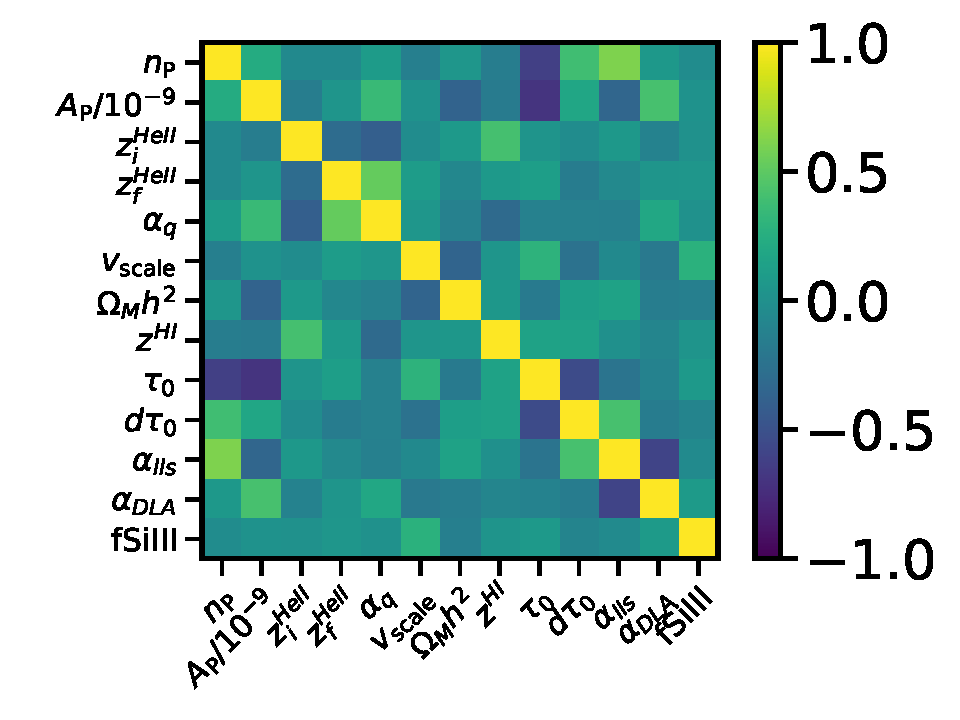
\includegraphics[width=0.98\textwidth]{figures/correlation_z26_46_t0.pdf}
    \caption{\label{fig:correlations}
    Correlation matrix between parameters for the chain using the flux power spectrum and mean IGM temperature for $z: 2.6-4.6$.
    }
\end{figure}
% Correlation matrix without T0
%           ns :  1.0000  0.2989 -0.0268 -0.0490  0.0257 -0.0754 -0.0491 -0.1703 -0.6291  0.3609  0.4835  0.1507 -0.0127
%           Ap :  0.2989  1.0000 -0.1286 -0.0670  0.2543  0.1259 -0.3552 -0.1103 -0.7505  0.1851 -0.4653  0.5361  0.0057
%        herei : -0.0268 -0.1286  1.0000  0.1633 -0.0118 -0.0476  0.0601  0.0165  0.0591 -0.2435  0.0829 -0.1175  0.0110
%        heref : -0.0490 -0.0670  0.1633  1.0000  0.0918 -0.0176 -0.0714 -0.0644  0.0628 -0.3173  0.0452 -0.1602 -0.0054
%       alphaq :  0.0257  0.2543 -0.0118  0.0918  1.0000  0.1144 -0.0463  0.0042 -0.0033 -0.1293 -0.1642  0.2450  0.0258
%          hub : -0.0754  0.1259 -0.0476 -0.0176  0.1144  1.0000 -0.1717  0.0392  0.1245 -0.1800 -0.0951 -0.1156  0.1681
%     omegamh2 : -0.0491 -0.3552  0.0601 -0.0714 -0.0463 -0.1717  1.0000  0.0952 -0.0590  0.1020  0.1259 -0.1542 -0.0753
%     hireionz : -0.1703 -0.1103  0.0165 -0.0644  0.0042  0.0392  0.0952  1.0000  0.1615  0.2233 -0.0266 -0.0099  0.0090
%         tau0 : -0.6291 -0.7505  0.0591  0.0628 -0.0033  0.1245 -0.0590  0.1615  1.0000 -0.4760 -0.0468 -0.2471  0.0572
%        dtau0 :  0.3609  0.1851 -0.2435 -0.3173 -0.1293 -0.1800  0.1020  0.2233 -0.4760  1.0000  0.3109 -0.0607 -0.0532
%        a_lls :  0.4835 -0.4653  0.0829  0.0452 -0.1642 -0.0951  0.1259 -0.0266 -0.0468  0.3109  1.0000 -0.6318 -0.0396
%        a_dla :  0.1507  0.5361 -0.1175 -0.1602  0.2450 -0.1156 -0.1542 -0.0099 -0.2471 -0.0607 -0.6318  1.0000  0.1124
%       fSiIII : -0.0127  0.0057  0.0110 -0.0054  0.0258  0.1681 -0.0753  0.0090  0.0572 -0.0532 -0.0396  0.1124  1.0000
% 
% Correlation matrix with T0
%           ns :  1.0000  0.2312 -0.0513 -0.0483  0.0943 -0.1385  0.0504 -0.1548 -0.6190  0.3904  0.6101  0.0683 -0.0274
%           Ap :  0.2312  1.0000 -0.1523  0.0397  0.3556  0.0219 -0.3646 -0.1661 -0.6959  0.1815 -0.3378  0.4202  0.0208
%        herei : -0.0513 -0.1523  1.0000 -0.2933 -0.3919 -0.0280  0.0721  0.4125  0.0368 -0.0293  0.0684 -0.1170  0.0152
%        heref : -0.0483  0.0397 -0.2933  1.0000  0.5297  0.1051 -0.0759  0.0796  0.1245 -0.1632 -0.0570  0.0413  0.0479
%       alphaq :  0.0943  0.3556 -0.3919  0.5297  1.0000  0.0539 -0.1226 -0.3059 -0.1224 -0.1207 -0.1296  0.2018  0.0096
%          hub : -0.1385  0.0219 -0.0280  0.1051  0.0539  1.0000 -0.3537  0.0459  0.2918 -0.2468 -0.0473 -0.1885  0.2780
%     omegamh2 :  0.0504 -0.3646  0.0721 -0.0759 -0.1226 -0.3537  1.0000  0.0606 -0.1742  0.1232  0.1544 -0.1543 -0.1355
%     hireionz : -0.1548 -0.1661  0.4125  0.0796 -0.3059  0.0459  0.0606  1.0000  0.1519  0.1456  0.0068 -0.0890  0.0370
%         tau0 : -0.6190 -0.6959  0.0368  0.1245 -0.1224  0.2918 -0.1742  0.1519  1.0000 -0.5392 -0.2271 -0.1165  0.0841
%        dtau0 :  0.3904  0.1815 -0.0293 -0.1632 -0.1207 -0.2468  0.1232  0.1456 -0.5392  1.0000  0.4176 -0.1630 -0.0950
%        a_lls :  0.6101 -0.3378  0.0684 -0.0570 -0.1296 -0.0473  0.1544  0.0068 -0.2271  0.4176  1.0000 -0.5910 -0.0462
%        a_dla :  0.0683  0.4202 -0.1170  0.0413  0.2018 -0.1885 -0.1543 -0.0890 -0.1165 -0.1630 -0.5910  1.0000  0.0880
%      fSiIII : -0.0274  0.0208  0.0152  0.0479  0.0096  0.2780 -0.1355  0.0370  0.0841 -0.0950 -0.0462  0.0880  1.0000

Figure~\ref{fig:correlations} shows the correlations between our parameters, for the chain using the flux power spectrum from $z=2.6 - 4.6$, as well as the mean IGM temperature.
Most correlations are weak.
We have deliberately chosen our pivot scale of $0.78$ h/Mpc to minimise the correlation between $A_P$ and $n_P$, and the correlation matrix confirms it is weak, with a correlation coefficient $r=0.2$. 
%Several of the stronger correlations arise from intrinsic degeneracies in the definition of the parameters and could in principle be reduced by modest redefinitions of pivot scales or pivot redshifts. 
There is a correlation between $\tau_0$ and $d\tau_0$ ($r=-0.54$), as the redshift bin which provides the strongest constraints on the optical depth is not exactly $z=3$.
The optical depth $\tau_0$ is anti-correlated with both $A_P$ ($r=-0.7$) and $n_P$ ($r=-0.62$) as its main effect is to change the amplitude of the flux power spectrum. 

There is a three-dimensional degeneracy between $\alpha_q$, $z_i^{HeII}$ and $z_i^{HeII}$ (see Figure~\ref{fig:correlations}), which allows a wide range of $\alpha_q$ to fit the flux power spectrum data, and is only broken by information from the thermal history.
Lower $\alpha_q$ corresponds to more heating from quasars during He~{\sc{ii}} reionization.
If He~{\sc{ii}} reionization starts earlier or ends later, the IGM requires more heating from quasars to match the observations, while the opposite is true for late starting, or early ending He~{\sc{ii}} reionization.
Appendix~\ref{sec:t0-only} shows the results of chains which include only the mean temperature data, which clearly shows this three-dimensional degeneracy: a slightly later start to Helium reionization would require less total heating and thus a higher value of $\alpha_q$. 
Several of these correlations could be broken by the inclusion of higher redshift thermal history data, or lower redshift flux power spectrum data. 

Finally, the abundance of Lyman Limit Systems, $\alpha_{LLS}$, exhibits several interesting correlations.
$\alpha_{LLS}$ is anti-correlated with $\alpha_{DLA}$ ($r=0.59$), as the flux power spectrum templates for strong absorbers have similar shapes in neighbouring column density bins.
$\alpha_{LLS}$ is also correlated with $n_P$ ($r=0.61$) and $d\tau_0$ ($r=0.42$), due to similarities in the shapes of their flux power spectrum templates.
The combination of the three-way correlation between $n_P$, $\alpha_{LLS}$ and $\tau_0$ is exploited by the chains to explain the inconsistent $z=2.2, 2.4$ flux power spectrum bins and drives the discrepant constraints these chains show.
This correlation may be reduced by the inclusion of extra small-scale data available in the DESI early data release.

%--------------------------------------------------------------------------------------------------
\section{Discussion}
\label{sec:discussion}

In this Section we discuss the implications of the results in Section~\ref{sec:results}. 
Section~\ref{sec:tension} discusses possible explanations for the internal tension in the data between $z = 2.2 - 2.4$ and $z \geq 2.6$.
Section~\ref{sec:comparison} compares our results to other datasets and earlier \Lya~analyses.
Section~\ref{sec:altlikelihood} discusses how our results are affected by modifications to our likelihood.

\subsection{The Tension in the Lowest Redshift Bins}
\label{sec:tension}

\begin{figure}
    \centering
    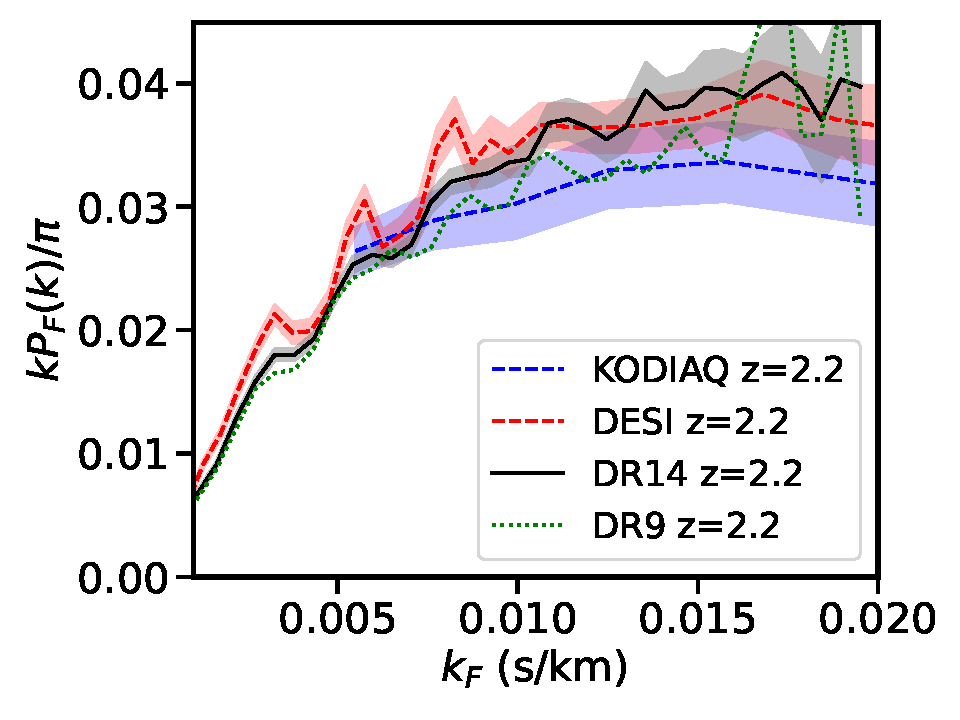
\includegraphics[width=0.45\textwidth]{figures/lymandata-z2.2.pdf}
    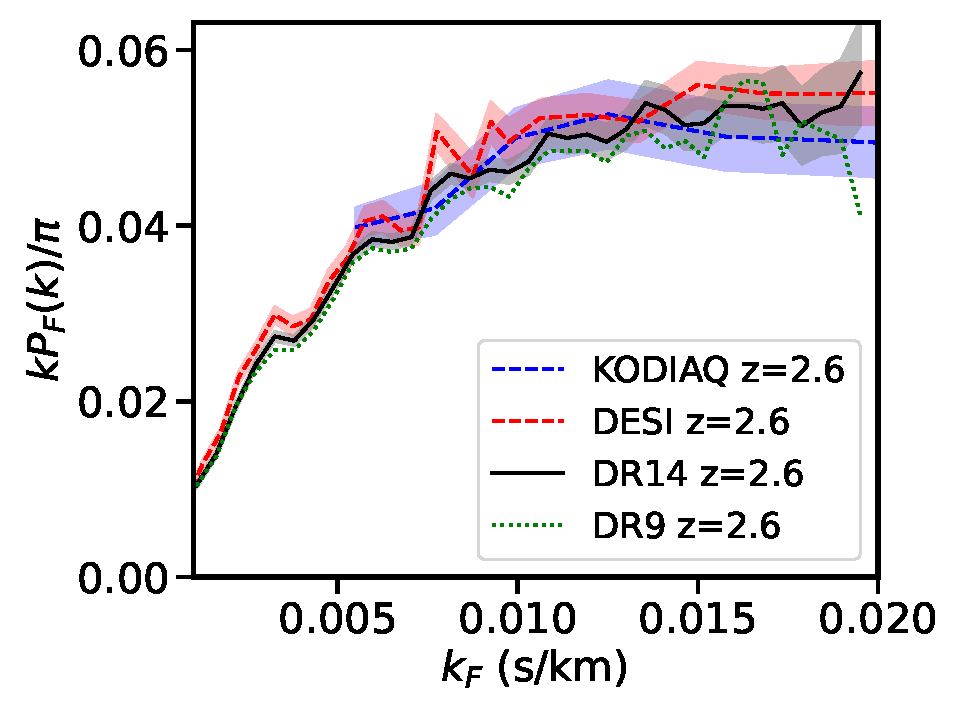
\includegraphics[width=0.45\textwidth]{figures/lymandata-z2.6.pdf}
    \caption{\label{fig:p1d_data}
    Observational 1D power spectrum data from SDSS DR14 (solid black) \protect\cite{2019JCAP...07..017C}, SDSS DR9 (green dotted) \protect\cite{2013A&A...559A..85P} and KODIAQ/SQUAD \protect\cite{2022MNRAS.509.2842K}.
    Filled bands show the range covered by diagonal elements of the covariance matrix.
    (Left) At $z=2.2$.
    (Right) At $z=2.6$.}
\end{figure}

In this Section, we discuss possible explanations for the internal tension between the flux power spectrum data at $z=2.2 - 2.4$ and $z \geq 2.6$.
There are two generic possibilities: either an important physical effect is missing from our simulation model, or there is a systematic in the dataset not captured by the systematic error budget. 

To evaluate the possibility of systematic error, we can look at independent measurements of the flux power spectrum on similar scales and at similar redshifts.
Figure~\ref{fig:p1d_data} shows different measurements of the 1D flux power, $P_F(k)$, at $z=2.2$ and $z=2.6$.
We show the results from SDSS DR14 \cite{2019JCAP...07..017C}, SDSS DR9 \cite{2013A&A...559A..85P}, a recent analysis using high resolution spectra from KODIAQ/SQUAD \cite{2022MNRAS.509.2842K}, and from DESI Early Data Release data (DESI EDR) \cite{2023arXiv230606316G}.
At $z=2.6$ (and higher redshift bins) all analyses are in reasonably good agreement, given their respective statistical errors.
However, this is not the case at $z=2.2$, where there is some discrepancy between SDSS (DR14 and DR9), DESI and KODIAQ.
SDSS DR14 and DR9 are in good agreement, and in Appendix \ref{sec:dr9_results} we show that the posterior parameter constraints also agree well. 

The KODIAQ flux power spectrum is lower by around $1-\sigma$ on the smallest scales measured by eBOSS, which could be due to the effect of continuum modelling in the KODIAQ data \cite{2022MNRAS.509.2842K}.
The DESI EDR data agrees well with eBOSS for $k > 0.01$ s/km, but is discrepant by $> 2 \sigma$ for $k < 0.01$ s/km.
This discrepancy is also present at $z=2.4$, and is discussed in the DESI EDR papers, see Ref.~\cite{2023arXiv230606311R}, Appendix D.
They ascribed $30\%$ of the difference to continuum fitting, but the origin of the rest is currently unclear.
Given the fairly large disagreements between different measurements at $z=2.2$, systematic error is a highly plausible explanation for the internal tension we find.
In future work we will combine our likelihood function with the DESI flux power spectra and investigate their cosmological implications.

We should also consider possible theoretical explanations.
Explanations rooted in alternative early Universe models seem a priori unlikely as they would have to cause an effect only for $z < 2.6$, when the Universe is known to be matter dominated. 
However, there are a few possible astrophysical explanations.
Feedback effects from AGN become increasingly important at low redshift.
It is possible that a stronger AGN feedback prescription than we use, or than is implemented in current cosmological simulation suites, could efficiently disrupt gas at $z < 2.6$ on small scales and explain these results.
Interestingly, such an AGN feedback model has recently been proposed as an explanation for the low value of $S_8 = \sigma_8 (\Omega_M/0.3)^{0.5}$ preferred by some weak lensing surveys \cite{2022MNRAS.516.5355A}, which matches our results.
However, Ref.~\cite{2023arXiv230706360T} examined a wide range of AGN feedback models, including some much more aggressive than those in PRIYA (or ASTRID).
None of these models can affect the $z=2.2$ flux power spectrum at the level required to explain these results (Tillman, private communication).

DLAs are important at low redshift, and do affect the slope of the flux power spectrum.
However, our simulations include a population of DLAs in good agreement with observations \cite{2023simsuite}, which are masked using the same procedure as the observational pipeline.
In addition, we include a free parameter to model the residual power from any DLAs not detected by eBOSS, and the posterior value for this free parameter is consistent with zero even when the $z=2.2$ data is included.
At low redshift, the \Lya~forest is increasingly contaminated by metal lines.
We include a simple prescription for \ion{Si}{III} and the inclusion of low redshift data does not drive the best-fit parameter for this model, preferring slightly less metal contamination.
However, it is possible that a more sophisticated model could help reduce the tension.

One interesting but entirely speculative possibility is suggested by the LLS abundance, $\alpha_{LLS}$, which is lower in the full redshift chains.
\cite{Prochaska:2009a} identified a systematic in the SDSS colour selection which causes quasar sightlines containing Lyman Limit Systems (LLS) to be preferentially selected for spectroscopic followup.
\cite{Worseck:2011} and \cite{Fumagalli:2013} showed that, due to the width of the $u$-band filter in SDSS, LLS are over-sampled for $z=2.5-3.6$ for all quasars in the redshift range $z=3.0-3.6$.
It is thus possible that $\alpha_{LLS}$ depends on the quasar (not absorber) redshift.
Note that the flux power spectrum we measure depends on the absorber redshift and so a simple redshift split would not detect this effect\footnote{We ran a chain with two $\alpha_{LLS}$ parameters for $z < 2.6$ and $z \geq 2.6$. The maximum likelihood for $\alpha_{LLS}$ at $z > 2.6$ was $\sim 2-\sigma$ larger than in the full redshift chain, and $n_P$ increased by $\sim 0.5\sigma$, but all other parameters were unchanged.}.
A check for colour selection systematics would involve the flux power spectrum being computed from two different quasar redshift bins.
%The \Lya forest probes marginally higher over-densities at low redshifts, so it is possible that a novel self-interacting dark matter model could be constructed which explains these observations, but it would have trouble matching cluster data (commented because I think the model would be a bit contrived).

\subsection{Comparison of the Posterior Constraints to Other Analyses}
\label{sec:comparison}

%Shift between DR9 and DR14 found in PD2020 but we don't (perhaps because the DLA model absorbs it).

%Other results: can compare only for the full redshift range.
%PD2020: ns low, sigma8 high, tau0 normal. We find tau0 high, sigma8 low, ns low. Quantitatively our results are more discrepant with Planck than theirs. Perhaps this is because their Taylor expansion tends to flatten gradients far from the central value, perhaps because we are measuring nP on small scales, not ns on large scales.
%PD2020 explicitly tested excluding the two lowest redshift bins and found no change in cosmological parameters. Not clear why.

It is interesting to compare the results of our chains to those of Ref.~\cite{2020JCAP...04..038P} (for DR14) and Ref.~\cite{2015JCAP...11..011P} (for DR9).
The most notable difference is that Ref.~\cite{2020JCAP...04..038P} tested excluding the lowest two redshift bins and found minimal change in the posteriors of their cosmological parameter.
This disagrees with our results.
We believe this discrepancy can be ascribed to our different treatment of nuisance parameters. Ref.~\cite{2020JCAP...04..038P} employed correction functions for supernova feedback from the OWLs simulation suite \cite{2013MNRAS.429.1734V} and for AGN feedback from the Horizon-AGN suite \cite{2020MNRAS.495.1825C}.
Each correction function is most significant at low redshift, and is included with a free amplitude parameter which is marginalised over.
In addition, earlier models were forced by computational limits to use the `splicing' technique of Ref.~\cite{2014JCAP...07..005B}.
In this model multiple simulation boxes with over-lapping scale ranges are combined to model the scales probed by the \Lya~forest.
A single larger simulation with $2048^3$ particles was used to generate a scale and redshift dependent correction function, and the amplitude of this correction was marginalised over with a Gaussian prior.

Our larger simulations can instead model all relevant scales in a single simulation and so do not need a free parameter for splicing.
In addition, we self-consistently incorporate models for stellar and AGN feedback and star formation into our simulations.
Thus the analysis of Ref.~\cite{2020JCAP...04..038P} differs from ours in that it has three nuisance parameters, each of which affects the lowest redshift bins most strongly and each of which is marginalised over in the chains.
Ref.~\cite{2015JCAP...02..045P} mentions that removing splicing reduces $n_s$ significantly (although the posterior value of the splicing correction is not reported), which is what we would expect if the splicing correction were absorbing an internal tension. 
Thus we believe that the $z=2.2$ and $z=2.4$ redshift bins contribute only marginally to the cosmological constraints in Ref.~\cite{2020JCAP...04..038P} and instead constrain splicing and AGN feedback. 
We should therefore compare the quantitative results of Ref.~\cite{2020JCAP...04..038P} to our reduced redshift chains. 

Ref.~\cite{2015JCAP...11..011P} find a mean optical depth of $\tau_{eff} (z=3) = 0.0025 \pm 0.0001$ and $d\tau = 3.734 \pm 0.015$ in DR9.
Ref.~\cite{2020JCAP...04..038P} do not report a value for $\tau_{eff}(z=3)$ from DR14, but we presume it is similar to that in DR9.
We define the mean optical depth relative to the power law $\tau_{eff} = 0.0023 (1+z)^{3.65}$, so that in our parameterization these constraints correspond to $\tau_0 = 1.09 \pm 0.05$ and $d\tau_0 = 0.084\pm 0.015$.
Their optical depth measurements are thus in good agreement with our measurements for the reduced redshift range of $z=2.6 - 4.6$. 

Ref.~\cite{2020JCAP...04..038P} found $n_s = 0.954 \pm 0.006$ for DR14 and $n_s = 0.938 \pm 0.010$ for DR9.
Meanwhile the power spectrum amplitude as measured by $\sigma_8$ is $0.826 \pm 0.02$ in DR14 and similar in DR9.
We find $n_P \sim 0.97$ and $\sigma_8 \sim 0.73$. Some of the differences between our constraints on $A_P$ and $\sigma_8$ are due to a lever arm effect: for $n_s < 1$ the power spectrum amplitude will be increased on larger scales and measuring $n_s$ will induce a correlation between $n_s$ and $\sigma_8$.

Ref.~\cite{2023arXiv230300746G} constrain the slope and amplitude of the linear matter power spectrum at $z=3$ using the reduced likelihood from Ref.~\cite{2023ApJ...944..223P}.
They use the full redshift range of the data, but without adding nuisance parameters.
Their best-fit parameters approximately correspond to $n_P \sim 0.93$ and $A_P \sim 1.5 \times 10^{-9}$, a low slope and low amplitude compared to Planck, and reasonably close to the results from our full redshift chain.

As shown in Appendix~\ref{sec:dr9_results}, we do not reproduce the $\sim 1\sigma$ shift in $n_s$ from DR9 to DR14 observed by Ref.~\cite{2020JCAP...04..038P}, and attributed by them to the different catalogues for masking DLAs and BAL.
Our DR9 and DR14 constraints are in very good agreement (as expected, since the two datasets have a large fraction of the spectra in common).
Our simulations include self-shielding of the gas following Ref.~\cite{Rahmati:2013} and a realistic DLA model, masked from the flux power spectrum in the same way as the observational data.
That the cosmological parameters are not affected by the change in DLA catalogue is reassuring, as it suggests that our analysis is indeed correctly marginalising over the uncertainty from DLAs.

%Notice that the average bias of forest gas without self-shielding is not the same as the average bias of forest gas with self-shielding and DLA masking \cite{2023MNRAS.524.1464P}. Furthermore, galaxy formation model changes which only affect dense gas cannot affect the \Lya flux power spectrum in our modelling and thus we are insensitive to the details of supernova feedback.

Rather than use effective broken power laws for the IGM thermal history as a function of redshift, we have explicit physical models for hydrogen and helium reionization, which include the scale-dependent effects of patchy reionization.
As shown in Figure~\ref{fig:temp_data}, the preferred IGM thermal history shows a temperature peak at $z=2.8$ and thus $T_0(z)$ cannot be described by a power law broken at $z=3$ as assumed in Ref.~\cite{2020JCAP...04..038P} and many earlier works.
Figure~\ref{fig:fps_data} shows that this does not affect the flux power spectrum on the scales measured by eBOSS.
However, DESI data will probe smaller scales, so it is not clear that this will be the case in future. 

%We do not include special parameters for the running $\alpha_s$ and neutrino mass $M_\nu$ in our emulator, preferring to model the effective amplitude and slope of the primordial power spectrum on the scales probed by the \Lya~forest, similarly to the reduced likelihood of Ref.~\cite{2023ApJ...944..223P} (but with parameters for the thermal history).

%Comparison to PD 2020: different model, no Taylor expansion but a LHS. No splicing, but multi-fidelity emulator. Correction for Sn from OWLS and AGN from the different simulation Horizon-AGN. We integrate both directly into our simulations. Our simulations include DLAs, star formation, galactic winds, AGN explicitly. No quick lyman alpha. Explicit helium and hydrogen reionization models which add a scale-dependent bias. No special parameters for alpha and Mnu in the emulator, instead we model them as changing nP and AP respectively. 
%The same SDSS DR14 dataset has been analysed by Ref.~\cite{2020JCAP...04..038P}. There are many differences in approach between our modelling and the earlier simulation models, as well as improvements driven by improved computation. Most significantly, our multi-fidelity emulation scheme \cite{2022MNRAS.509.2551H} allows us to build a model for the \Lya~forest which fully resolves the forest in a $120$ Mpc/h box. 

%Similarly, we do not use the simple second-order gradient expansion of the dependence of the flux power spectrum on cosmological parameters used in Ref.~\cite{2020JCAP...04..038P} and earlier works, but instead build an emulator on a parameter grid sampled using a Latin Hypercube, which better captures correlations between parameters \cite{2019JCAP...02..050B}. 


\subsection{Likelihood Modifications}
\label{sec:altlikelihood}

We also considered modifications to the likelihood not shown here.
First, we increased the observational uncertainty from eBOSS by a uniform factor of two.
This increased the posterior uncertainties, but did not significantly resolve the internal tension at low redshift (as this is many $\sigma$).
We also considered removing the high redshift data, with $z > 3.8$, as is done in some earlier analyses \cite{2011MNRAS.413.1717B}.
We found that this made little difference as the statistical errors in the high redshift data are large and so they provide little information. 
%We did confirm that the high redshift bins are not in tension with the low redshift data. 
We considered removing the largest and smallest scales with cuts in $k$.
Several of the smallest scale bins are highly correlated, and so removing them either led to very poor constraints or had small effects, depending on the scale cut.
Removing the largest bins on the largest scales increased the posterior uncertainty, but did not noticeably shift the posteriors.
Thus none of these checks show any evidence for an internal tension between scales.

We tested whether a second mean flux rescaling slope would improve the fit to the observed \lya forest flux power (Figure~\ref{fig:fps_data}), especially at lower redshifts and smaller scales.
To do this, we added a second mean flux slope to the MCMC sampled parameters, and assigned each to a specific redshift range (we tested this using a redshift pivot of $z=3$ and $z=3.6$).
Posterior constraints on the other parameters from a chain run using the second mean flux slope were unaffected and the fit was not improved.
